\chapter{Podstawowe pojęcia}
\label{c2}

W danym rozdziale zostaną zawarte podstawowe pojęcia i mechanizmy używane przez aplikację App Inventor. Ideą tutaj jest przypomnienie oraz przypliżenie ważnych terminów informatycznych.

\section{App Inventor}
\label{c21}

W grudniu 2013 roku został wydany App Inventor w wersji drugiej. Starsza wersja została nazwana jako Classic. Oba narzędzia są bardzo podobne jednak projekty stworzone w starszej wersji nie mogą zostać zaimportowane do nowszej. W danej pracy magisterskiej skupienie zostało na nowej wersji App Inventora.

App Inventor jest to system, który pozwala na tworzenie aplikacji używając jedynie przeglądarki internetowej. Jest to aplikacja internetowa, umożliwiająca zrobienie programu, przez użytkowników mających bardzo małe pojęcie o programowaniu. 

Potencjał aplikacji jest bardzo duży. Można to zauważyć patrząc na ilość aktywnych użytkowników. W maju 2014 roku, liczba aktywnych użytkowników wynosiła 87tys. tygodniowo. Ilość zarejestrowanych to 1,9mln w 195 krajach. Użytkownicy ci stworzyli razem 4,7mln projektów.\cite{article:appinventor1}

\section{Główne komponenty}
\label{c22}

App Inventor celowo ułatwia programowanie poprzez wizualizację tworzonych komponentów i intuicyjny interfejs. App Inventor składa się z 3 głównych komponentów jakimi są:
\begin{itemize}
\item App Inventor Designer
\item App Inventor Blocks Editor
\item Android Device Emulator
\end{itemize}

\subsection{App Inventor Designer}
\label{c221}

Jednym z głównych widoków jakie można używać jest widok Designera. Projektowanie interfejsu użytkownika polega na przeciąganiu komponentów z dostępnej palety, wliczając w to także niewidoczne komponenty takie jak sensory. W tym widoku można również zmieniać właściwości obiektów, które zostały stworzone. Między innymi istnieje możliwość zmiany położenia, wielkości, układu (pionowy, poziomy).

Designer jest zaprojektowany jako zwykła aplikacja internetowa. Tak więc uruchamia się go, jak zwykłą stronę internetową wpisując jej adres www.

\begin{figure}[th] 
\centering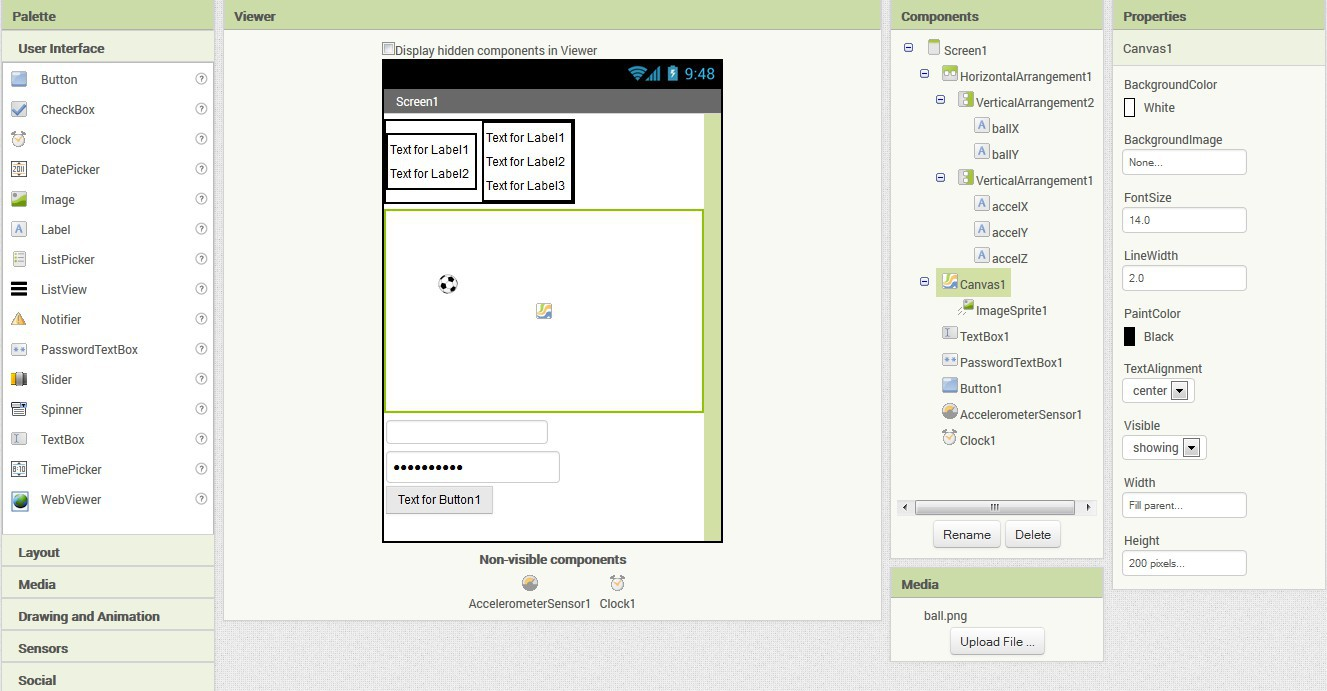
\includegraphics[width=10cm]{figures/designer}
\caption{App Inventor Designer}
\end{figure}

\subsection{App Inventor Blocks Editor}
\label{c222}

Drugim widokiem jest Blocks Editor. Zachowanie aplikacji zostaje tutaj zaprogramowane poprzez połączenie odpowiednich bloków. Istnieje możliwość korzystania z bardziej generalnych komponentów, a także z bardziej specyficznych. Dla każdego komponentu, który został stworzony w interfejsie graficznym (Designerze) są dostępne bloki mówiące, co tak naprawdę jest możliwe do zrobienia. Wygląda to w ten sposób, że komponenty są przciągane z dostępnej palety medotą "przeciągnij i upuść", a następnie łączone jak puzzle.

Ta część aplikacji normalnie reprezentowana jest przez kod napisany przez programistę. Więc napisanie zachowania aplikacji odbywa się poprzez łączenie puzzli, bez znajomości języka Java.

\begin{figure}[th] 
\centering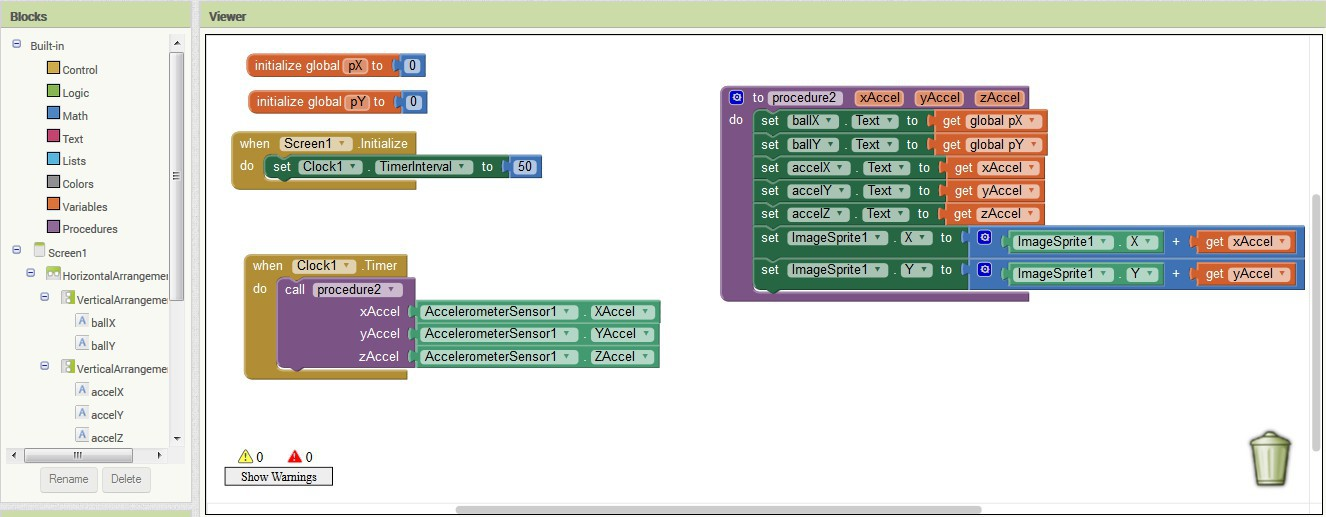
\includegraphics[width=10cm]{figures/editor}
\caption{App Inventor Blocks Editor}
\end{figure}

\subsection{Android Device Emulator}
\label{c223}

Android Device Emulator jest to emulator telefonu lub tabletu. Jest to wirtualna wersja smartphonu, w której znajdują się obsługa dotyku ekranu, przyciski systemowe oraz typowe funkcje.

Zmiany, które zostają wprowadzone, natychmiast reflektują na działanie aplikacji. Nie ma potrzeby jakiejkolwiek kompilacji i uruchamiania aplikacji od nowa. Jeżeli aplikacja zostanie uruchomiana, kompilacja zmienionych fragmentów oraz zainstalowanie ich na emulatorze dzieje się w czasie rzeczywistym. Jest to bardzo wygodna opcja budowania aplikacji i testowania jej. Zmiany, które zrobimy są od razu widoczne na ekranie.

\begin{figure}[th] 
\centering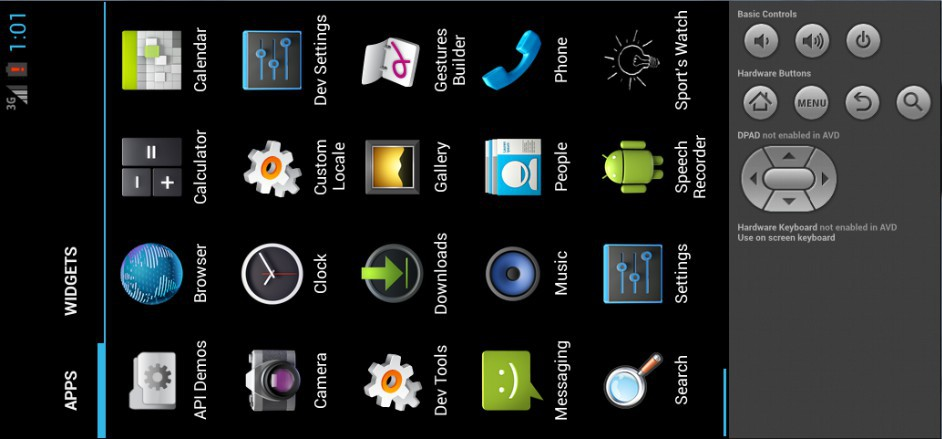
\includegraphics[width=10cm]{figures/emulator}
\caption{Android Device Emulator}
\end{figure}


\subsection{Android SDK}

Android SDK - jest to zestaw narzędzi programistycznych, które są oferowane dla programistów, chcących tworzyć aplikacje na platformę Android. Jest on modularny, poprzez SDK Managera, możemy zainstalować, tylko te komponenty, które nas interesują. 

\subsection{SDK Tools}

Android SDK dzieli się na dwie części SDK Tools oraz Platform Tools. Najważniejsze narzędzia wchodzące w skład pierwszej części to:
\begin{itemize}
\item AVD Manager - odpowiedzialny za zarządzanie wirtualnymi urządzeniami z systemem operacyjnym android. Jest to najłatwiejsza i najwygodniejsza opcja stworzenia nowego wirtualnego urządzenia i odpowiedniego sparametryzowania go.
\item SDK Manager - wspomniany wyżej, odpowiedzialny za instalację modułów, które nas interesują
\item Emulator - emualtor systemu android, stworzony przez AVD Managera
\item Dalvik Debug Monitor (DDMS) \label{ddms}- jest to narzędzie pomocne w debugowaniu aplikacji. Dostarcza on takich funkcji jak przekierowanie portów, przechwyt obrazu na urządzeniu, informacje o wątkach, stosie, a także o metodach, które są uruchomione jeżeli włączymy ich profilowanie.
\end{itemize}

\subsection{Platform Tools}

\begin{itemize}
\item Android Debug Bridge \label{adb}- narzędzie pozwalające na komunikację z podłączonym urządzeniem. Jest także używany do instalacji i uruchamiania aplikacji. Składa się z 2 części, klienta i serwera, które komunikują się ze sobą.
\end{itemize}

\subsection{Apktool}

Jest to narzędzie do tak zwanej inżynierii odwrotnej (\english{Reverse engineering}). Umożliwia ono dekodowanie programu do prawie oryginalnej formy. Następnie, po dokonaniu pewnych modyfikacji umożliwia ono zbudowanie aplikacji z powrotem do wyjściowej formy.\cite{doc:apktool}

\subsection{Keystore}

Jest to repozytorium przechowujące certyfikaty bezpieczeństwa. Do zarządzania certyfikatami istnieje narzędzie o nazwie keytool. Umożliwia ono użytkownikom zarządzanie prywatnymi/publicznymi kluczami, certyfikatami jak i podpisem elektornicznym.\cite{doc:keytool}

\subsection{Jarsigner}

System android wymaga, aby aplikacje na nim instalowane były cyfrowo podpisane. Dzięki temu system może zweryfikować autora aplikacji. Podpisywanie aplikacji dzielimy na 2 sposoby: tryb debugowania (\english{Debug mode})oraz tryb wydania (\english{Release mode}). Przy korzystaniu ze zintegrowanego środowiska programistycznego zwykle aplikacja zostaje cyfrowo podpisana automatycznie, podczas instalacji jej na telefonie. Jarsigner umożliwia popisanie aplikacji manualnie, korzystając z lini poleceń.
